\subsubsection{BRAM}
\index{BRAM (package)}
%\index{Xilinx!BRAM (package)}
\label{sec-BRAM}

{\bf Package}


\begin{verbatim}
import BRAM :: * ;
\end{verbatim}


{\bf Description}

The \te{BRAM} package provides types, interfaces, and modules
to support FPGA BlockRams.  The BRAM modules include FIFO wrappers to
provide implicit conditions for proper flow control for the BRAM
latency.    Specific 
tools may determine whether modules are mapped to appropriate BRAM
cells during synthesis.

The \te{BRAM} package is open-sourced and can be modified by the user.
The low-level wrappers to the BRAM Verilog and Bluesim modules, which
are not open-sourced and cannot be modified,  are
provided in the \te{BRAMCore} package, Section \ref{sec-BRAMCore}.

{\bf Types and type classes}
\index{BRAM\_Configure@\te{BRAM\_Configure} (type)}
\paragraph{BRAM\_Configure}

The \te{BRAM\_Configure} structure specifies the underlying  modules and their
attributes for instantiation.    Default values for the BRAM are
defined with the \te{DefaultValue} instance and can easily be modified.

\begin{center}
\begin{tabular}{|p {.8 in}|p {.7 in}| p {2.2 in}|p {1.5in}|}
\hline
\multicolumn{4}{|c|}{BRAM\_Configure Structure}\\
\hline
Field &Type &Description& Allowed or\\
&&& Recommended Values\\
\hline
\hline
\te{memorySize}&Integer&Number of words in the BRAM   &\\
\hline
\te{latency}&Integer&Number of stages in the read&1 (address is registered)\\
&&&2 (address and data are registered)\\
\hline
\te{loadFormat}&LoadFormat&Describes the  load file&\te{None}\\
&&&\te{tagged Hex} {\em filename}  \\
&&&\te{tagged Binary} {\em filename}\\
\hline
\te{outFIFODepth}&Integer&The depth of the BypassFIFO after the BRAM
for the BRAMServer module&latency+2 \\
\hline
\multicolumn{2}{|l|}{\te{allowWriteResponseBypass}}&&\\
&Bool&Determines if write responses can directly be enqueued in the
output fifo (\te{latency = 0} for write).&\\
\hline
\end{tabular}
\end{center}

The size of the BRAM is determined by the \te{memorySize} field given
in number of words.  The width of a word is determined by the
polymorphic type \te{data} specified in the BRAM interface. If
the \te{memorySize} field is 0, then  memory size = $ 2^{n}$, where
\te{n} is the number 
of address bits determined from the address type.

The \te{latency} field has two valid values; \te{1} indicates that the
address on the read is registered, \te{2} indicates that both the
address on the read input and the  data on the read output  are
registered.  When latency = 2, the components in the dotted box in
Figure \ref{bram} are included.

The \te{outFIFODepth} is  used to determine the depth of the Bypass
FIFO after the BRAM in  the  \te{mkBRAMServer} module.  This value
should be \te{latency + 2} to allow full pipeline behavior.

The \te{allowWriteResponseBypass} field, when \te{True}, 
specifies that the write response is issued on the same cycle as the
write request.  If \te{False}, the write reponse is pipelined, which is 
 the same behavior as the read request. When \te{True}, the schedule
 constraints between \te{put} and \te{get} are \te{put SBR get}.
 Otherwise, the annotation is \te{get CF put} (no constraint).



\begin{verbatim}
typedef struct {Integer      memorySize ;
                Integer      latency ;              // 1 or 2 can extend to 3
                LoadFormat   loadFormat;            // None, Hex or Binary
                Integer      outFIFODepth;
                Bool         allowWriteResponseBypass;
               } BRAM_Configure ;
\end{verbatim}

The \te{LoadFormat} defines the type of the load file (\te{None},
 \te{Hex} or \te{Binary}). The type \te{None} is used when there is no
 load file.  When the type is \te{Hex} or \te{Binary}, the
 name of the load file is provided as  a \te{String}. 

\begin{verbatim}
typedef union tagged {
                      void None;
                      String Hex;
                      String Binary;
   } LoadFormat
deriving (Eq, Bits);
\end{verbatim}

The default values are defined in this package using the
\te{DefaultValue} instance for \te{BRAM\_Configure}.  You can modify
the default values by changing this instance or by modifying specific
fields in your design.

\begin{center}
\begin{tabular}{|p{1.8 in}|p {.8 in}| p{.5  in}| p {2.2in}|}
\hline
\multicolumn{4}{|c|}{Values defined in defaultValue}\\
\hline
Field&Type& Value&Meaning\\
\hline
\hline
\te{memorySize}&Integer&0& $ 2^{n}$, where \te{n} is the number
of address bits\\
\hline
\te{latency}&Integer&1&address is registered\\
\hline
\te{outFIFODepth}&Integer&3&latency + 2\\
\hline
\te{loadFormat}&\te{LoadFormat}  &None&no load file is used\\
\hline
\te{allowWriteResponseBypass}&Bool&False&the write response is pipelined\\
\hline
\end{tabular}
\end{center}

\begin{verbatim}
instance DefaultValue #(BRAM_Configure);
   defaultValue = BRAM_Configure {memorySize        : 0
                                 ,latency           : 1 // No output reg
                                 ,outFIFODepth      : 3
                                 ,loadFormat        : None
                                 ,allowWriteResponseBypass  : False  };
endinstance
\end{verbatim}

To modify a default configuration for your design, set the field you want to
change to the new value.  Example:
\begin{verbatim}
BRAM_Configure cfg = defaultValue ;     //declare variable cfg 
             cfg.memorySize = 1024*32 ; //new value for memorySize
             cfg.loadFormat = tagged Hex "ram.txt";  //value for loadFormat
BRAM2Port#(UInt#(15), Bit#(16)) bram <- mkBRAM2Server (cfg) ;
                                        //instantiate 32K x 16 bits BRAM module
\end{verbatim}


\index{BRAMRequest@\te{BRAMRequest} (type)}

\paragraph{BRAMRequest}

The \te{BRAM} package defines  2  structures for a BRAM request:
\te{BRAMRequest}, and the byte enabled version \te{BRAMRequestBE}.

\begin{center}
\begin{tabular}{|p {1.2 in}|p {.5 in}| p {3.2 in}|}
\hline
\multicolumn{3}{|c|}{ BRAMRequest Structure}\\
\hline
Field &Type &Description\\
\hline
\hline
\te{write}&Bool&Indicates whether this operation is a  write (\te{True)} or
a read (\te{False}).\\
\hline
\te{responseOnWrite}&Bool&Indicates whether a response should be
received from this write command \\
\hline
\te{address}&\te{addr}&Word address of the read or write\\
\hline
\te{datain}&\te{data}&Data to be written.  This field is ignored for reads.\\
\hline
\end{tabular}
\end{center}

\begin{verbatim}
typedef struct {Bool write;
                Bool responseOnWrite;
                addr address;
                data datain;
               } BRAMRequest#(type addr, type data) deriving(Bits, Eq);
\end{verbatim}



\paragraph{BRAMRequestBE}
The  structure \te{BRAMRequestBE} allows for the byte enable signal.

\begin{center}
\begin{tabular}{|p {1.2 in}|p {.5 in}| p {3.2 in}|}
\hline
\multicolumn{3}{|c|}{ BRAMRequestBE Structure}\\
\hline
Field &Type &Description\\
\hline
\hline
\te{writeen}&\te{Bit\#(n)}&Byte-enable indicating whether this operation is
a write (n != 0) or a read (n = 0).\\
\hline
\te{responseOnWrite}&Bool&Indicates whether a response should be
received from this write command \\
\hline
\te{address}&\te{addr}&Word address of the read or write\\
\hline
\te{datain}&\te{data}&Data to be written.  This field is ignored for reads.\\
\hline
\end{tabular}
\end{center}



\begin{verbatim}
typedef struct {Bit#(n) writeen;
                Bool    responseOnWrite;
                addr    address;
                data    datain;
               } BRAMRequestBE#(type addr, type data, numeric type n) deriving (Bits, Eq);
\end{verbatim}

{\bf Interfaces and Methods}

%\index{BRAM\_PORT@\te{BRAM\_PORT} (interface type)}
\index{BRAM@\te{BRAM} (interface type)}
%\index{BRAM\_DUAL\_PORT@\te{BRAM\_DUAL\_PORT} (interface type)}

The interfaces for the BRAM are built on the \te{Server} interface
defined in the \te{ClientServer} package, Section
\ref{lib-clientserver}.  Some type aliases specific to the BRAM are
defined here.

BRAM Server and Client interface types :
\begin{verbatim}
typedef Server#(BRAMRequest#(addr, data), data) BRAMServer#(type addr, type data);
typedef Client#(BRAMRequest#(addr, data), data) BRAMClient#(type addr, type data);
\end{verbatim}

 Byte-enabled BRAM Server and  Client interface types:
\begin{verbatim}
typedef Server#(BRAMRequestBE#(addr, data, n), data) 
        BRAMServerBE#(type addr, type data, numeric type n);
typedef Client#(BRAMRequestBE#(addr, data, n), data) 
        BRAMClientBE#(type addr, type data, numeric type n);
\end{verbatim}


The \te{BRAM} package defines 1 and 2 port interfaces, with
write-enabled and byte-enabled versions.  Each BRAM  port interface contains a
\te{BRAMServer\#(addr, data)} subinterface and a clear action, which clears
the output FIFO of any pending requests.  The data in the BRAM is not cleared.

\begin{center}
\begin{tabular}{|p{.7 in}|p{2.1 in}|p{2.7 in}|}
\hline
\multicolumn{3}{|c|}{BRAM1Port Interface}\\
\multicolumn{3}{|c|}{1 Port BRAM Interface}\\
\hline
Name & Type&Description \\
\hline
\hline 
\te{portA}&\te{BRAMServer\#(addr, data)} &Server subinterface\\
\hline
\te{portAClear}&Action&Method to clear the portA output FIFO \\
\hline
\end{tabular}
\end{center}

\begin{verbatim}
interface BRAM1Port#(type addr, type data);
   interface BRAMServer#(addr, data) portA;
   method Action portAClear;
endinterface: BRAM1Port
\end{verbatim}

\begin{center}
\begin{tabular}{|p{.7 in}|p{2.1 in}|p{2.7 in}|}
\hline
\multicolumn{3}{|c|}{BRAM1PortBE Interface}\\
\multicolumn{3}{|c|}{Byte enabled 1 port BRAM Interface}\\
\hline
Name & Type&Description \\
\hline
\hline 
\te{portA}&\te{BRAMServerBE\#(addr, data, n)} &Byte-enabled server subinterface\\
\hline
\te{portAClear}&Action&Method to clear the portA output FIFO \\
\hline
\end{tabular}
\end{center}


\begin{verbatim}
interface BRAM1PortBE#(type addr, type data, numeric type n);
   interface BRAMServerBE#(addr, data, n) portA;
   method Action portAClear;
endinterface: BRAM1PortBE
\end{verbatim}

\begin{center}
\begin{tabular}{|p{.7 in}|p{2.1 in}|p{2.7 in}|}
\hline
\multicolumn{3}{|c|}{BRAM2Port Interface}\\
\multicolumn{3}{|c|}{ 2 port BRAM Interface}\\
\hline
Name & Type&Description \\
\hline
\hline 
\te{portA}&\te{BRAMServer\#(addr, data)} &Server subinterface for
port A\\
\hline
\te{portB}&\te{BRAMServer\#(addr, data)} &Server subinterface for port
B\\
\hline
\te{portAClear}&Action&Method to clear  the port A output FIFO \\
\hline
\te{portBClear}&Action&Method to clear the port B output FIFO \\
\hline
\end{tabular}
\end{center}

\begin{verbatim}
interface BRAM2Port#(type addr, type data);
   interface BRAMServer#(addr, data) portA;
   interface BRAMServer#(addr, data) portB;
   method Action portAClear;
   method Action portBClear;
endinterface: BRAM2Port
\end{verbatim}

\begin{center}
\begin{tabular}{|p{.7 in}|p{2.1 in}|p{2.7 in}|}
\hline
\multicolumn{3}{|c|}{BRAM2PortBE Interface}\\
\multicolumn{3}{|c|}{Byte enabled 2 port BRAM Interface}\\
\hline
Name & Type&Description \\
\hline
\hline 
\te{portA}&\te{BRAMServerBE\#(addr, data, n)} &Byte-enabled server
subinterface for port A\\
\hline
\te{portB}&\te{BRAMServerBE\#(addr, data, n)} &Byte-enabled server
subinterface for port B\\
\hline
\te{portAClear}&Action&Method to clear  the  portA output FIFO \\
\hline
\te{portBClear}&Action&Method to clear the portB output FIFO \\
\hline
\end{tabular}
\end{center}

\begin{verbatim}
interface BRAM2PortBE#(type addr, type data, numeric type n);
   interface BRAMServerBE#(addr, data, n) portA;
   interface BRAMServerBE#(addr, data, n) portB;
   method Action portAClear;
   method Action portBClear;
endinterface: BRAM2PortBE
\end{verbatim}



{\bf Modules}

The BRAM modules defined in the \te{BRAMCore} package (Section
\ref{sec-BRAMCore}) are wrapped with control logic to turn the BRAM
into a server, as shown in Figure \ref{bram}.  The BRAM Server modules
include an output FIFO and 
logic to control its loading and to avoid overflow.  A single port,
single clock byte-enabled version is provided as well as 2 port and
dual clock  write-enabled versions.


\begin{figure}[ht]
\begin{center}
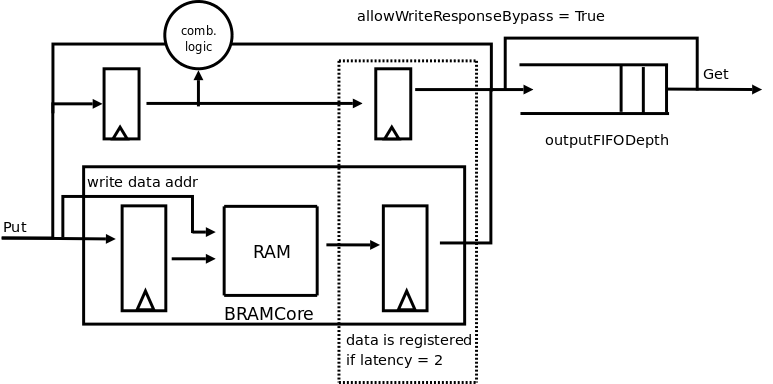
\includegraphics[width = 4 in]{LibFig/BRAM}
\caption{1 port of a BRAM Server}
\label{bram}
\end{center}
\end{figure}



\index{mkBRAM1Server@\te{mkBRAM1Server} (module)}
\index[function]{BRAM!mkBRAM1Server}
\label{sec-BRAM1Server}
\begin{tabular}{|p{1.4 in}|p{4.2 in}|}
\hline
& \\
\te{mkBRAM1Server}&BRAM Server module including an output FIFO and
logic to control  loading and to avoid overflow. \\
\cline{2-2}
& \begin{libverbatim}
module mkBRAM1Server #( BRAM_Configure cfg ) 
                      ( BRAM1Port #(addr, data) )
   provisos(Bits#(addr, addr_sz),
            Bits#(data, data_sz),
            DefaultValue#(data) );
\end{libverbatim}
\\
\hline
\end{tabular}
\label{sec-BRAM1ServerBE}
\index{mkBRAM1ServerBE@\te{mkBRAM1ServerBE} (module)}
\index[function]{BRAM!mkBRAM1ServerBE}

\begin{tabular}{|p{1.4 in}|p{4.2 in}|}
\hline
& \\
\te{mkBRAM1ServerBE}&Byte-enabled BRAM Server module. \\
\cline{2-2}
& \begin{libverbatim}
module mkBRAM1ServerBE #( BRAM_Configure cfg ) 
                        ( BRAM1PortBE #(addr, data, n) )
   provisos(Bits#(addr, addr_sz),
            Bits#(data, data_sz),
            Div#(data_sz, n, chunk_sz),
            Mul#(chunk_sz, n, data_sz), 
            DefaultValue#(data) );
\end{libverbatim}
\\
\hline
\end{tabular}


\index{mkBRAM2Server@\te{mkBRAM2Server} (module)}
\index[function]{BRAM!mkBRAM2Server}

\begin{tabular}{|p{1.4 in}|p{4.2 in}|}
\hline
& \\
\te{mkBRAM2Server}&2 port BRAM Server module. \\
\cline{2-2}
& \begin{libverbatim}
module mkBRAM2Server #( BRAM_Configure cfg ) 
                      ( BRAM2Port #(addr, data) )
   provisos(Bits#(addr, addr_sz),
            Bits#(data, data_sz),
            DefaultValue#(data) );
\end{libverbatim}
\\
\hline
\end{tabular}

\begin{tabular}{|p{1.4 in}|p{4.2 in}|}
\hline
& \\
\te{mkBRAM2ServerBE}&Byte-enabled 2 port BRAM Server module. \\
\cline{2-2}
& \begin{libverbatim}
module mkBRAM2ServerBE #( BRAM_Configure cfg ) 
                        ( BRAM2PortBE #(addr, data, n) )
   provisos(Bits#(addr, addr_sz),
            Bits#(data, data_sz),
            Div#(data_sz, n, chunk_sz),
            Mul#(chunk_sz, n, data_sz) );
\end{libverbatim}
\\
\hline
\end{tabular}



\index{mkSyncBRAM2Server@\te{mkSyncBRAM2Server} (module)}
\index[function]{BRAM!mkSyncBRAM2Server}

\begin{tabular}{|p{1.4 in}|p{4.2 in}|}
\hline
& \\
\te{mkSyncBRAM2Server}&2 port, dual clock,  BRAM Server module. The
\te{portA} subinterface and \te{portAClear} methods are in the
\te{clkA} domain;
the \te{portB} subinterface and \te{portBClear} methods are in the \te{clkB}
domain. \\
\cline{2-2}
& \begin{libverbatim}
(* no_default_clock, no_default_reset *)
module mkSyncBRAM2Server #( BRAM_Configure cfg,
                           Clock clkA, Reset rstNA,
                           Clock clkB, Reset rstNB
                           ) (BRAM2Port #(addr, data) )
   provisos(Bits#(addr, addr_sz),
            Bits#(data, data_sz),
            DefaultValue#(data) );

\end{libverbatim}
\\
\hline
\end{tabular}

\index{mkSyncBRAM2ServerBE@\te{mkSyncBRAM2ServerBE} (module)}
\index[function]{BRAM!mkSyncBRAM2ServerBE}

\begin{tabular}{|p{1.4 in}|p{4.2 in}|}
\hline
& \\
\te{mkSyncBRAM2ServerBE}&2 port, dual clock, byte-enabled BRAM Server
module. The 
\te{portA} subinterface and \te{portAClear} methods are in the
\te{clkA} domain;
the \te{portB} subinterface and \te{portBClear} methods are in the \te{clkB}
domain. \\
\cline{2-2}
& \begin{libverbatim}
(* no_default_clock, no_default_reset *)
module mkSyncBRAM2ServerBE #(BRAM_Configure cfg,
                             Clock clkA, Reset rstNA,
                             Clock clkB, Reset rstNB )
                          (BRAM2PortBE #(addr, data, n))
   provisos(Bits#(addr, addr_sz),
            Bits#(data, data_sz),
            Div#(data_sz, n, chunk_sz),
            Mul#(chunk_sz, n, data_sz) );
\end{libverbatim}
\\
\hline
\end{tabular}




{\bf Example: Using a BRAM}
\begin{verbatim}
import BRAM::*;
import StmtFSM::*;
import Clocks::*;

function BRAMRequest#(Bit#(8), Bit#(8)) makeRequest(Bool write, Bit#(8) addr, Bit#(8) data);
   return BRAMRequest{
                      write: write,
                      responseOnWrite:False,
                      address: addr,
                      datain: data
                      };
endfunction

(* synthesize *)
module sysBRAMTest();
    BRAM_Configure cfg = defaultValue;
    cfg.allowWriteResponseBypass = False;
    BRAM2Port#(Bit#(8), Bit#(8)) dut0 <- mkBRAM2Server(cfg);
    cfg.loadFormat = tagged Hex "bram2.txt";
    BRAM2Port#(Bit#(8), Bit#(8)) dut1 <- mkBRAM2Server(cfg);

   //Define StmtFSM to run tests
   Stmt test =
   (seq
       delay(10);
       ...
       action
          dut1.portA.request.put(makeRequest(False, 8'h02, 0));
          dut1.portB.request.put(makeRequest(False, 8'h03, 0));
       endaction
       action 
          $display("dut1read[0] = %x", dut1.portA.response.get);
          $display("dut1read[1] = %x", dut1.portB.response.get);
       endaction
       ...
       delay(100);
    endseq);
   mkAutoFSM(test);
endmodule
\end{verbatim}
